%%%%%%%%%%%%%%%%%%%%%%%%%%%%%%%%%%%%%%%%%%%%%%%%%%%%%%%%%%%%%%%%%%%%%%%%%%%%%%%%
%%
%%   BornAgain User Manual
%%
%%   homepage:   http://www.bornagainproject.org
%%
%%   copyright:  Forschungszentrum Jülich GmbH 2015
%%
%%   license:    Creative Commons CC-BY-SA
%%   
%%   authors:    Scientific Computing Group at MLZ Garching
%%               C. Durniak, M. Ganeva, G. Pospelov, W. Van Herck, J. Wuttke
%%
%%%%%%%%%%%%%%%%%%%%%%%%%%%%%%%%%%%%%%%%%%%%%%%%%%%%%%%%%%%%%%%%%%%%%%%%%%%%%%%%


\chapter{Wave propagation through multilayers}  \label{sec:Multilayers}

This chapter describes how to calculate the coherent wave solution for neutrons incident on a multilayered sample. In the first section, only scalar interactions will be considered. The second part uses a spinor and matrix formalism to account for neutron polarization.

%%%%%%%%%%%%%%%%%%%%%%%%%%%%%%%%%%%%%%%%%%%%%%%%%%%%%%%%%%%%%%%%%%%%%%%%%%%%%%%%
\section{Multilayer systems}
%%%%%%%%%%%%%%%%%%%%%%%%%%%%%%%%%%%%%%%%%%%%%%%%%%%%%%%%%%%%%%%%%%%%%%%%%%%%%%%%

\index{Multilayer systems}%

%===============================================================================
\subsection{DWBA}
%===============================================================================

In many applications of GISAS,
the investigated sample consists of a number of distinct layers.
For the time being,
no other systems are supported in BornAgain.\footnote
{Please contact us if need arises for modelling systems with
smoothly varying~$\nz(z)$.
\index{Refractive index!graded}%
}
Within one layer~$j$, the average refractive index is constant,
$\nz(z)=\nzj$ for $z\in\mathcal{Z}_j$, where
$\mathcal{Z}_j$ denotes an interval on the vertical coordinate axis.
Within a layer,
the downward and upward propagating waves are plane,
\begin{equation}
  \Psi^\pm_{wj}(\r)=A^\pm_{wj}\e^{i\k^\pm_{wj}\r}.
\end{equation}
\nomenclature[2j020]{$j$}{Index of layer in multilayer sample}%
\nomenclature[2a123 2w010 2j010 \pm]{$A^\pm_{wj}$}{Amplitude of the plane wave $\Psi^\pm_{wj}(\r)$}%
\index{Fresnel coefficients}%
\index{Transmission|see {Fresnel coefficients}}%
\index{Reflection|seealso {Fresnel coefficients}}%
Here and in the following,
the index~$w$ can take the values i and~f.
The amplitudes $A$ are often written with distinct letters
T and~R to designate the transmitted or reflected beam,
\begin{equation}
  T_{wj} := A^-_\text{wj},\quad
  R_{wj} := A^+_\text{wj}.
\end{equation}
The wave vector can be decomposed as
\begin{equation}
  \k^\pm_{wj}= \k_{\parallel w} \pm k_{\perp wj}\v{\hat z}.
\end{equation}
\nomenclature[2z060]{$\v{\hat z}$}{Unit vector along the sample normal}%
\nomenclature[2k043 2w010 2j010 \pm]{$\k^\pm_{wj}$}{Wave vector of the plane wave $\Psi^\pm_{wj}(\r)$}%
As explained in connection with~(\ref{Ekpar}),
the in-plane wave vector $\k_{\parallel w}$ remains constant
across layer interfaces.
The vertical wavenumber is obtained from (\ref{Ewavez}),
\begin{equation}
  k_{\perp wj} = \sqrt{K^2 \nzj - k_{\parallel w}^2}.
\end{equation}
Restricting (\ref{EBornQ}) to one layer,
the Fourier transform of the refractive index fluctuations
shall be written as
\begin{equation}\label{Echij}
  \chi_j(\v{q})
  := \int_{z\in\mathcal{Z}_j}\!\d^3r\, \e^{i\v{q}\,\r}\chi(\r).
\end{equation}
\nomenclature[1χ032 2j010 2q040]{$\chi_j(\v{q})$}{Fourier transform of the perturbation potential $\chi(\r)$, evaluated in one sample layer}%
We can then write the DWBA transition matrix~(\ref{EtmDWBAsum}) as
a sum over all layers,
\index{Distorted-wave Born approximation!multilayer}%
\Highlight{\Box{
\begin{equation}\label{EtmDWBAft}
  \bra \Psi_\text{f}|\chi|\Psi_\text{i}\ket
  = \sum_{j} \sum_{\pm_\text{f}} \sum_{\pm_\text{i}}
    A^\pm_{\text{i}j} A^{\pm *}_{\text{f}j}
     \chi_j(\k^\pm_{\text{i}j} - \k^\pm_{\text{f}j}).
\end{equation}
}}

%===============================================================================
\subsection{Transmission and reflection coefficients}
%===============================================================================

The coefficients $A^\pm_{wj}$
can be calculated using the Parratt formalism \cite{Par54}
or the matrix method \cite{BoWo99}.

..... And how are they actually computed in BornAgain? .....

%===============================================================================
\subsection{Embedded particles}
%===============================================================================

\index{Particles!embedded|(}%
\index{Nanoparticles|see {Particles}}%
\index{Mesoparticles|see {Particles}}%
In many important GISAS applications,
fluctuations of the refractive index are due to particles
of mesoscopic size (nanometer to micrometer).
These particles are either embedded into a material layer,
or attached to the surface of the sample.
In BornAgain, the latter case must be construed as a special form of the former
by defining an extra layer on top of the regular surface that
consists of vacuum (or air) with embedded particles.

For the time being,
we consider scattering from only one layer;
therefore we can omit the layer index~$j$ from the following considerations.
The layer has a thickness~$d$ and contains $N$ particles per area~$A$.
% hence the particles have a number density of $\nu=N/(Ad)$.
Particle~$i$, located at $\r_i$,
has a volume~$V_i$ and scattering length density~$\rho_i(\r-\r_i)$.
Outside the volumes occupied by particles,
the scattering length has a constant density of~$\chi_0$.
The average scattering length density of the entire layer is then
\begin{equation}\label{Emulaynav}
  \begin{split}
  \overline{\rho}
      &= \frac{\sum_i \int_{V_i}\!\d^3r\; \rho_i(\r-\r_i)
               + (Ad-\sum_i V_i)\rho_0}
             {Ad}\\[1em]
      &= \rho_0 + \frac{\sum_i \int_{V_i}\!\d^3r\, [\rho_i(\r-\r_i)-\rho_0]}
             {Ad}
  \end{split}
\end{equation}
To predict the GISAS pattern,
we need to compute the Fourier transform (\ref{Echij}) of
$\chi(\r)=\rho(\r)-\overline{\rho}$.
There are two contributions to the Fourier integrand:
from the embedded particles, and from the embedding matrix,
which has the structure of an Emmental cheese:
homogeneous except for holes where the particles are.
Fortunately, we do not need to compute the Fourier transform
of the cheese:
Analogous to (\ref{Emulaynav}),
we can rearrange the Fourier integral as
\begin{equation}\label{Echijre}
  \chi_j(\v{q})
  = \int_{z\in\mathcal{Z}_j}\!\d^3r\, \e^{i\v{q}\,\r}
    \left\{ \left(\rho_0-\overline{\rho}\right)
           + \sum_i \left[(\rho_i(\r-\r_i)-\rho_0\right] \right\}
  =: \chi^0_j + \chi^\text{p}_j.
\end{equation}
The first term is the shape transform of the entire layer
\begin{equation}
  \chi^0_j(\v{q})
   = \int_{z\in\mathcal{Z}_j}\!\d^3r\, \e^{i\v{q}\,\r}
      \left(\rho_0-\overline{\rho}\right)
   = \delta(\v{q}_\parallel)\;d\;\text{sinc}(q_\parallel d/2).
\end{equation}
For the second term,
we abbreviate
\begin{equation}
  \delta\rho_i(\r):=\rho_i(\r)-\rho_0,
\end{equation}
and we introduce the form factor of a single particle
\begin{equation}
  F_i(\v{q}) := \int\!\d^3r\, \e^{i\v{q}\,\r} \delta\rho_i(\r).
\end{equation}
We can then rearrange to obtain
\begin{equation}
  \chi^\text{p}_j(\v{q})
  = \sum_i \e^{i\v{q}\,\r_i} F_i(\v{q}).
\end{equation}
Implemented single-particle form fators $F_i(\v{q})$
are listed in great detail in chapter~\ref{sec:FormFactors}.
The positional phase factors $\e^{i\v{q}\,\r_i}$
can give rise to inter-particle interference patterns
that are discussed in chapter~\ref{sec:Assemblies}.

%===============================================================================
\subsection{OLD STUFF}
%===============================================================================

... the same techniques as demonstrated in section \ref{sec:ba} can be applied, leading to the following expression for the expectation value of the scattering cross-section:
\begin{align*}
  & \bra \frac{d\sigma}{d\Omega}(\k_\text{i},\k_\text{f}) \ket_{\text{Off-specular}}  \\
  & = \sum_\alpha p_\alpha \left\lvert \curlf_\alpha(\k_{j,i},\k_{j,f}, R_{\alpha,z})\right\rvert ^2 + \frac{\rho_S}{S}\sum_{\alpha,\beta} p_\alpha p_\beta \curlf_\alpha (\k_{j,i},\k_{j,f}, R_{\alpha,z})\curlf_\beta^*(\k_{j,i},\k_{j,f}, R_{\beta,z}) \\
  & \times \iint_S d^2\r_\alpha^\parallel d^2\r_\beta^\parallel \ppcf{\alpha}{\beta}{R^\parallel} \exp \left[ i\v{q}_{j\parallel}\cdot (\r_\alpha^\parallel - \r_\beta^\parallel ) \right].
\end{align*}

The main differences with respect to the cross-section in the Born approximation are:
\begin{enumerate}
  \item The particle form factor now consists of a more complex expression and now depends on both incoming and outgoing wave vectors and also on the $z$-coordinate of the particle;
  \item Since the $z$-coordinate of the particles is implicitly included in its formfactor, the position integrals only run over $x$- and $y$-coordinates and the volume and density gets replaced with the surface area and surface density respectively.
\end{enumerate}

%%%%%%%%%%%%%%%%%%%%%%%%%%%%%%%%%%%%%%%%%%%%%%%%%%%%%%%%%%%%%%%%%%%%%%%%%%%%%%%%
\section{Geometry of the sample}
%%%%%%%%%%%%%%%%%%%%%%%%%%%%%%%%%%%%%%%%%%%%%%%%%%%%%%%%%%%%%%%%%%%%%%%%%%%%%%%%

\noindent The geometry used to describe the sample is
shown in Fig.~\ref{fig:multil3d}. The $z$-axis is perpendicular to the sample's
surface and pointing upwards. The $x$-axis  is perpendicular to the
detector plane. The input and the
scattered output beams are each characterized by two angles
$\alpha_i$, $\phi_i$ and $\alpha_f$, $\phi_f$, respectively. Our choice of orientation for the
angles $\alpha_i$ and $\alpha_f$ is so that they are positive
as shown in Fig.~\ref{fig:multil3d}. \\

\begin{figure}[ht]
  \centering
    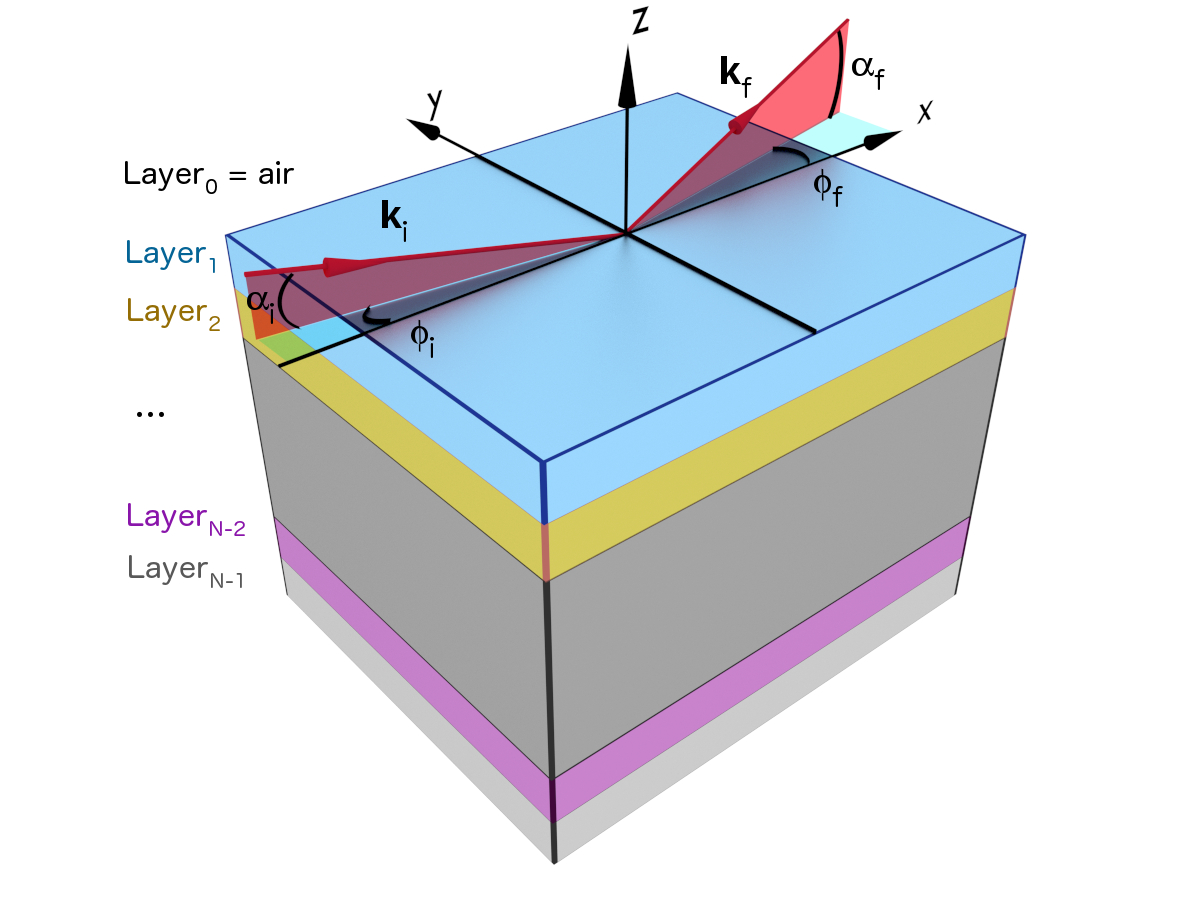
\includegraphics[clip=, width=120mm]{fig/drawing/setup_multilayer.jpg}
  \caption[Representation of the scattering geometry.]{Representation of the scattering geometry. $n_j$ is
    the refractive index of layer $j$ and $\alpha_i$ and $\phi_i$ are the incident
    angles of the wave propagating. $\alpha_f$ is the exit angle with respect to the sample's surface and
$\phi_f$ is the scattering angle with respect to the scattering
plane. }
  \label{fig:multil3d}
\end{figure}

The layers are defined by their thicknesses (parallel to the
$z$-direction), their possible
roughnesses (equal to 0 by default) and the
materials they are made of. They have an infinite extension in the $x$ and $y$
directions. And, except for roughness, their interfaces are plane and
perpendicular to the $z$-axis. There is also no limitation to the
number of layers that could be defined in \BornAgain. Note that the
thickness of the top and bottom layer are not defined.

%\ImportantPoint{Remark:}{Order of layers: \\
%When assembling the sample, the layers are defined from top to
%bottom. So in most cases the first layer will be the air layer.}\\

The nanoparticles are characterized by their form factors
(\textit{i.e.} the Fourier transform of the shape function - see Appendix~\ref{app:ff} for a list of form factors implemented in \BornAgain) and the composing material. The number of input parameters for the form factor depends on the particle symmetry; it ranges from one parameter for a sphere (its radius) to three for an ellipsoid (its three main axis lengths).
  
By placing the particles
inside or on top of a layer, we impose their vertical positions, whose
values correspond to the bottoms of the particles. The in-plane distribution of particles is linked with the way the
particles interfere with each other. It is therefore implemented
when dealing with the interference function.

%\ImportantPoint{Remark:}{Depth of particles\\
%The vertical positions of particles in a layer are given in relative
%coordinates. For the top layer, the bottom corresponds to
%\texttt{depth}=0. But for all the other layers, it is the top of the
%layer which corresponds to \texttt{depth}=0.}\\

\index{Refractive index}
\index{Index of refraction|see {Refractive index}}
The complex refractive index associated with a layer or a particle
is written as $n=1-\delta +i\beta$,
with $\delta, \beta \in \mathbb{R}$.
In our program, we input $\delta$ and $\beta$ directly.


\noindent The input beam is assumed to be monochromatic without any
spatial divergence.\\ %\textbf{polarization term?}

%\newcommand{\vect}[1]{\ensuremath{\mathbf{#1}}}
%\newcommand{\unitvec}[1]{\ensuremath{\widehat{\vect{#1}}}}
%\newcommand{\altc}[1]{\ensuremath{\widetilde{#1}}}
%\newcommand{\beq}{\begin{equation}}
%\newcommand{\eeq}{\end{equation}}
\renewcommand{\u}[1]{\underline{#1}}
\newcommand{\uu}[1]{\underline{\underline{#1}}}
\renewcommand{\t}{\uparrow}
\renewcommand{\d}{\downarrow}

%\renewcommand\Im{\operatorname{Im}}
%\renewcommand\Re{\operatorname{Re}}


%%%%%%%%%%%%%%%%%%%%%%%%%%%%%%%%%%%%%%%%%%%%%%%%%%%%%%%%%%%%%%%%%%%%%%%%%%%%%%%%
\section{Basic formalism for scalar index of refraction}
%%%%%%%%%%%%%%%%%%%%%%%%%%%%%%%%%%%%%%%%%%%%%%%%%%%%%%%%%%%%%%%%%%%%%%%%%%%%%%%%

In this section,
we investigate refraction by a multilayer system
with flat interfaces and with scalar refraction indices.
We first develop the basic formalism
without absorption, and far from total reflection conditions.
Absorption, total reflection and evanescent waves
will be discussed in subsection~\ref{s:complex}.
In section~\ref{s:pol},
we generalize the formalism to include
polarization-dependent interaction.

Polarized neutron propagation at glancing incidence
in multilayer systems has been studied by Spiering and Deak [...],
using Abeles' matrix formalism and matrix exponentials.
In Abeles' formalism [],
plane waves are parametrized by $\psi$ and $\partial_z\psi$.
We prefer a parametrization (\ref{Epsiz})
by the amplitudes of forward and backward propagating plane waves,
which is mathematically simpler,
and allows a more direct physical interpretation.

%-------------------------------------------------------------------------------
\subsection{Wave equation for a basic multilayer model}
%-------------------------------------------------------------------------------

The geometry for reflection by a multilayer sample is shown in figure~\ref{fig:multil3d}. Here we only consider specular reflection, hence the azimuthal angle $\phi_f = 0$.

All layer interfaces are assumed to be perfectly smooth.
All layers are homogenous; layer~$i$ has the complex refractive index~$n_i$.
Layer~0 is the air or vacuum on top of the sample;
layer~$N$ is the substrate; these two layers are assumed semi-inifinite.
We first consider scalar interactions.
Polarization-dependent reflection
will be discussed in section~\ref{s:pol}. 

Within one layer,
stationary wave propagation with given frequency,
hence with fixed vacuum wave number~$K$,
obeys the differential equation
\begin{equation}\label{Escalar_wave}
\left(\Delta + K^2 n_i^2 \right) \psi(\r) = 0.
\end{equation}
At interfaces between layers,
the wave function $\psi(\r)$ and its first derivative
$\Nabla\psi(\r)$ must evolve continuously.


%-------------------------------------------------------------------------------
\subsection{Wave propagation within one layer}
%-------------------------------------------------------------------------------

Since our multilayer model has infinite extension
in $x$ and $y$--directions, we can factorize
$\psi(\r)$, and assume plane-wave propagation for
the in-plane component $\r_\parallel$ (\ref{Ewave3}):
\begin{equation}\label{Ewave3dup}
\psi(\r) = \psi(z) \e^{i \k_\parallel\r_\parallel}.
\end{equation}
From the continuity conditions we infer that $\k_\parallel$
is constant across layers.
The wave equation~(\ref{Escalar_wave})
reduces to a one-dimensional equation in~$z$ [see (\ref{Ewavez})]
\begin{equation}\label{Ewavezdup}
\left(\partial_z^2 + K^2n_i^2 - k_\parallel^2 \right) \psi(z) = 0,
\end{equation}
which is solved by
\begin{equation}\label{Epsiz}
  \psi_i(z) = a_i\e^{ik_{\perp i}(z-z_i)} + b_i\e^{-ik_{\perp i}(z-z_i)},
\end{equation}
where $z_i$ is the coordinate of the \textit{bottom} interface
of layer $i$,
introduced here as a constant offset for later convenience.
In the case of the semi-infinite bottom layer~$N$,
$z_N$ can be chosen arbitrarily.

Inserting (\ref{Epsiz}) into (\ref{Ewavezdup}),
we obtain the dispersion relation
\begin{equation}\label{Edisp}
  k_\parallel^2 + k_{\perp i}^2 = K^2 n_i^2.   
\end{equation}
If $n_i$ is real and $k_\parallel<K n_i$,
this is just the Pythagorean equation
for the perpendicular components of either of
the two wave vectors:
vector $\k_\pm=\k_\parallel \pm k_{\perp i}\v{\hat z}$.
They correspond to the two summands in (\ref{Epsiz}),
and describe plane waves propagating upwards or downwards.
These waves have glancing angles
\begin{equation}\label{Edef_alpha}
  \alpha_i:=\arctan(k_{\perp i}/k_\parallel).  
\end{equation}
Equivalently,
\begin{equation}
  k_\parallel=K n_i \cos\alpha_i. 
\end{equation}
Since $k_\parallel$ is constant across layers,
we have
\begin{equation}\label{ESnell}
  n_i \cos\alpha_i = \text{the same for all }i,
\end{equation}
which is Snell's refraction law.

For later convenience we abbreviate
\begin{equation}\label{Edef_f}
f_i := \sqrt{ n_i^2 - n_0^2 \cos^2\alpha_0 },
\end{equation}
which is a combination of material parameters ($n_0$, $n_i$)
and a geometric parameter ($\alpha_0$) that describes the incident beam.
If $n_i$ is real, and the argument of the square root nonnegative,
we simply have $f_i=n_i\sin\alpha_i$.
However, using $f_i$ allows for later generalizations
to cope with absorbing media or with total reflection and evanescent waves.
The wave number in (\ref{Epsiz}) can now be written as
\begin{equation}\label{EkKf}
  k_{\perp i} = K f_i.
\end{equation}


%-------------------------------------------------------------------------------
\subsection{Wave propagation across layers}
%-------------------------------------------------------------------------------

In this section,
the continuity of $\psi(z)$ and $\partial_z\psi(z)$ at layer interfaces
is used to derive a recursion rule
for the coefficients $a_i$ and $b_i$ of (\ref{Epsiz}).
At the \textit{bottom} interface of layer~$i=0,\ldots,N-1$,
continuity requires
\begin{equation}\label{Econtcond}
  \begin{array}{lcl}
            \psi_{i}(z_i)&=&\psi_{i+1}(z_{i+1}+d_{i+1}),\\
            \partial_z\psi_{i}(z_i)&=&\partial_z\psi_{i+1}(z_{i+1}+d_{i+1}),
  \end{array}
\end{equation}
  where
\begin{equation}
  d_i:=z_{i-1}-z_{i}
\end{equation}
is the thickness of layer~$i$.
With the solution (\ref{Epsiz}), conditions (\ref{Econtcond}) become
\begin{equation}\label{Econt2}
  \begin{array}{lclclcl}
  a_i &+& b_i,
  &=&
  a_{i+1}\e^{iKf_{i+1}d_{i+1}} &+& b_{i+1}\e^{-iKf_{i+1}d_{i+1}},
  \\
  a_i f_i  &-& b_i f_i,
  &=&
 a_{i+1}\e^{iKf_{i+1}d_{i+1}} f_{i+1} &-& b_{i+1}\e^{-iKf_{i+1}d_{i+1}} f_{i+1}.
  \end{array}
\end{equation}
We introduce the vector notation
\begin{equation}\label{Evecc}
  c_i := \left( \begin{array}{c}a_i\\b_i\end{array} \right),
\end{equation}
to write (\ref{Econt2}) as
\begin{equation}\label{EFcFDc}
  F_i c_i = F_{i+1} D_{i+1} c_{i+1}
\end{equation}
with the matrices
\begin{equation}
  F_i := \left(\begin{array}{cc}1&1\\f_i&-f_i\end{array}\right)\text{, and }
  D_i := \left(\begin{array}{cc}\delta_i&0\\0&\delta_i^*\end{array}\right),
\end{equation}
and the phase factor
\begin{equation}
   \delta_i := \e^{iKf_id_i}.
\end{equation}
We define the transfer matrix
\begin{equation}\label{Edef_M}
  M_i
  := F_{i-1}^{-1}F_i D_i,
\end{equation}
to obtain the recursion 
\begin{equation}\label{EcMc}
  c_i = M_{i+1} c_{i+1}.
\end{equation}
Straightforward computation yields
\begin{equation}
  M_i
   = \frac{1}{2f_{i-1}}
   \left(\begin{array}{cc}
       \delta_i(f_{i-1}+f_{i})&\delta_i^*(f_{i-1}-f_{i})\\
       \delta_i(f_{i-1}-f_{i})&\delta_i^*(f_{i-1}+f_{i})
   \end{array}\right)
   = \frac{1}{2}
   \left(\begin{array}{cc}
       \delta_i(1+\rho_{i})&\delta_i^*(1-\rho_{i})\\
       \delta_i(1-\rho_{i})&\delta_i^*(1+\rho_{i})
   \end{array}\right)
\end{equation}
with the ratio
\begin{equation}
  \rho_i := \frac{f_{i}}{f_{i-1}}.
\end{equation}
The recursion starts from the semi-infinite substrate layer~$N$
where there is no upwards propagating wave, hence $a_N=0$.
For layer~$i$, the solution is
\begin{equation}\label{Eci}
  c_i
  =
  M_{i+1}.... M_{N} c_N.  % TODO restore \cdots
\end{equation}

%-------------------------------------------------------------------------------
\subsection{Currents}
%-------------------------------------------------------------------------------

Currents shall be computed in relative units as
\begin{equation}
  \v{J}:=\psi^*(\r)\frac{\Nabla}{2i}\psi(\r)+\text{c.c.}
\end{equation}
We are interested in the component $J_z$.
With (\ref{Epsiz}),
we obtain in layer~$i$
\begin{equation}\label{EJperp}
  \begin{array}{lcl}
  J_{zi} &=& \frac{1}{2}
  \left( a_i^*\e^{-ik_{\perp i}(z-z_i)} + b_i^*\e^{ik_{\perp i}(z-z_i)} \right)
  k_{\perp i}
  \left( a_i\e^{ik_{\perp i}(z-z_i)} - b_i\e^{-ik_{\perp i}(z-z_i)} \right)
  +\text{c.c.}\\[2ex]
  &=& \left( |a_i|^2 - |b_i|^2 \right) K f_i,
  \end{array}
\end{equation}
provided $k_{\perp i}$ is real.
Obviously,
the $|a_i|^2$ term is due to the upward beam
and the $|b_i|^2$ term to the downward beam.

In the absence of absorption we expect that the net current
is the same in all layers.
We verify this as follows.
Using the vector notation~(\ref{Evecc}),
we write~(\ref{EJperp}) as a sesquilinear form
\begin{equation}
  J_{zi}
  = c_i^\dagger \left(\begin{array}{cc}Kf_i&0\\0&-Kf_i\end{array}\right) c_i.
\end{equation}
Using the recursion (\ref{EcMc}) for $c_i$,
we obtain a recursion for $J_{zi}$:
\begin{equation}\label{EJrec}
  \begin{array}{lcl}
    J_{zi} &=&
    c_{i}^\dagger
    \left(\begin{array}{cc}Kf_{i}&0\\0&-Kf_{i}\end{array}\right) c_{i}
    \\[3ex]
    &=&
    c_{i+1}^\dagger M_{i+1}^\dagger
    \left(\begin{array}{cc}Kf_{i}&0\\0&-Kf_{i}\end{array}\right)
    M_{i+1}c_{i+1}
    \\[3ex]
    &=&
    c_{i+1}^\dagger
    \left(\begin{array}{cc}Kf_{i+1}&0\\0&-Kf_{i+1}\end{array}\right)
    c_{i+1}
    \\[3ex]
    &=&
    J_{z,i+1},
  \end{array}
\end{equation}
which means that the net current is constant.

For a single interface between two semi-infinite media,
wave amplitudes are related by
\begin{equation}
    \left(\begin{array}{c}a_0\\b_0\end{array}\right)
  = M_1
    \left(\begin{array}{c}0\\b_1\end{array}\right)
  = \frac{\delta_1^* b_1}{2 f_0}
    \left(\begin{array}{c}f_0-f_1\\f_0+f_1\end{array}\right).
\end{equation}
The reflectivity of the interface is
\begin{equation}\label{ER01}
  R={\left|\frac{a_0}{b_0}\right|}^2
   ={\left|\frac{f_0-f_1}{f_0+f_1}\right|}^2,
\end{equation}
which agrees with Fresnel's result for $s$-polarized light.


%-------------------------------------------------------------------------------
\subsection{Damped waves in absorbing media
  or under total reflection conditions}\label{s:complex}
%-------------------------------------------------------------------------------

If layer~$i$ absorbs radiation,
its index of refraction $n_i$ has a positive imaginary component.
By~(\ref{Edisp}),
$k_\parallel^2+k_{\perp i}^2$ then also has a positive imaginary component.
From the continuity of $\psi$ and $\Nabla\psi$ across layer interfaces
it still follows that $\k_\parallel$ is constant.
We assume that the top layer~0 is not absorbing.
Hence $\k_\parallel$ is real.
To fulfill~(\ref{Edisp}),
it is necessary that $k_{\perp i}$
has a positive imaginary component.
In consequence,
the intensities of the forward and backward travelling beams (\ref{Epsiz})
decrease exponentially in~$\pm z$.

Snell's law of refraction (\ref{ESnell})
cannot be fulfilled if
\begin{equation}\label{Etotrefcond}
  n_i<n_0\cos\alpha_0.  
\end{equation}
In this case, total reflection occurs at the top interface of layer~$i$,
accompanied by an evanescent wave within layer~$i$.
Strictly speaking,
total reflection is only possible if layer~$i$ is not absorbing.
Otherwise, some intensity would be dissipated by the evanescent wave,
and the reflection would not be total.
Also, the unequality~(\ref{Etotrefcond}) is undefined
if $n_i$ has an imaginary component.

With definition~(\ref{Edef_f}),
total reflection occurs if $f_i$ is a pure imaginary number.
For an absorbing medium, $f_i$ has a positive imaginary part
and a non-zero real part.
Therefore it is appropriate to treat total reflection as a special
case of refraction by a medium with complex~$f_i$.

For complex $f_i$,
the theory developed above
remains applicable, with the following exceptions:
The geometric interpretation of the wave vectors $\k_\pm$
in Eqs.~(\ref{Edef_alpha}--\ref{ESnell}) is untenable,
and the computation of currents in
Eqs.~(\ref{EJperp}--\ref{EJrec}) is invalid because it
relies on $\Im k_{\perp i}=0$.


%-------------------------------------------------------------------------------
\subsection{Numerical considerations}
%-------------------------------------------------------------------------------

...



%%%%%%%%%%%%%%%%%%%%%%%%%%%%%%%%%%%%%%%%%%%%%%%%%%%%%%%%%%%%%%%%%%%%%%%%%%%%%%%%
\section{Reflection with polarization-dependent interactions}\label{s:pol}
%%%%%%%%%%%%%%%%%%%%%%%%%%%%%%%%%%%%%%%%%%%%%%%%%%%%%%%%%%%%%%%%%%%%%%%%%%%%%%%%

%\cite{Deak_ppt, PhysRevB.76.224420, Deak2001113, PhysRevB.53.6158}.
%\cite{RevModPhys.23.287}

%-------------------------------------------------------------------------------
\subsection{Wave equation and propagation within one layer}
%-------------------------------------------------------------------------------

To allow for polarization-dependent interactions,
we replace the squared index of refraction $n^2$
by $1+\uu\chi$, where $\uu\chi$ is a $2\times 2$ susceptibility matrix.
The wave equation (\ref{Escalar_wave}) for layer~$i$ becomes
\begin{equation}\label{Ewaveqp}  
(\Delta +K^2 +K^2 \uu\chi_i) \u\psi(\r)= 0,
\end{equation}
where $\u\psi(\r)$ is a two-component spinor wave function,
with components $\psi_\t(\r)$ and~$\psi_\d(\r)$.
At interfaces between layers,
both spinor components of $\u\psi(\r)$ and $\Nabla\u\psi(\r)$
must evolve continuously.

The reasons for the factorization (\ref{Ewave3}) still apply,
and so we can write
\begin{equation}\label{Ewave3p}
\u\psi(\r) = \u\psi(z) \e^{i \k_\parallel\r_\parallel}.
\end{equation}
As before, $\k_\parallel$ is constant across layers.
The wave equation~(\ref{Ewaveqp}) reduces to 
\begin{equation}\label{Ewavezp}
\left(\partial_z^2 + K^2 + K^2\uu\chi_i - k_\parallel^2 \right) \u\psi(z) = 0.
\end{equation}
We abbreviate
\begin{equation}
  \uu H_i := K^2(1+\uu\chi_i)-k_\parallel^2
\end{equation}
so that the wave equation becomes simply
\begin{equation}\label{Ewaveqp2}
  \left(\partial_z^2 + \uu H_i\right) \u\psi(z) = 0.
\end{equation}
The solution is
\begin{equation}\label{Epsizp}
  \u\psi_i(z)
  = \sum_{j=1}^2 \u x_{ij}\left(\alpha_{ij}\e^{i p_{ij}(z-z_i)}
                            + \beta_{ij}\e^{-i p_{ij}(z-z_i)}\right),
\end{equation}
where the $\u x_{ij}$ are eigenvectors of $\uu H_i$
with eigenvalues $p_{ij}^2$:
\begin{equation}
  \left( -p_{ij}^2 + \uu H_i \right) \u x_{ij} = 0
   \;\text{ for }\;j=1,2.
\end{equation}
In a reproducible algorithm,
the eigenvectors $\u x_{ij}$ must be chosen according to some arbitrary
normalization rule,
for instance
\begin{equation}
  |\u x_{ij}|=1,\quad x_{ij\t} \text{ real and nonnegative}.
\end{equation}
Similarly,
a rule is needed how to handle the case of one degenerate eigenvalue,
which includes in particular the case of scalar interactions.


%-------------------------------------------------------------------------------
\subsection{Wave propagation across layers}
%-------------------------------------------------------------------------------

Generalizing (\ref{Evecc}),
we introduce the coefficient vector
\begin{equation}
  c_i := {(\alpha_{i1}, \alpha_{i2}, \beta_{i1}, \beta_{i2})}^\text{T}.
\end{equation}
To match solutions for neighboring layers,
continuity is requested for both spinorial components
of $\u\psi$ and $\Nabla\u\psi$.
As before (\ref{EFcFDc}), we have at the bottom of layer~$i$
\begin{equation}\label{EFcFDcp}
  F_i c_i = F_{i+1} D_{i+1} c_{i+1},
\end{equation}
where the matrices are now
\begin{equation}
  F_i := \left(\begin{array}{cccc}
    x_{i1\t}      &x_{i2\t}     &x_{i1\t}       &x_{i2\t}       \\
    x_{i1\d}      &x_{i2\d}     &x_{i1\d}       &x_{i2\d}       \\
    x_{i1\t}p_{i1}&x_{i2\t}p_{i2}&-x_{i1\t}p_{i1}&-x_{i2\t}p_{i2}\\
    x_{i1\d}p_{i1}&x_{i2\d}p_{i2}&-x_{i1\d}p_{i1}&-x_{i2\d}p_{i2}
  \end{array}\right)
\end{equation}
and
\begin{equation}
  D_i := \text{diag}(\delta_{i1}, \delta_{i2}, \delta_{i1}^*, \delta_{i2}^*)
\end{equation}
with the phase factor
\begin{equation}
   \delta_{ij} := \e^{ip_{ij}d_i}.
\end{equation}
Note that matrix $F_i$ has the block form
\begin{equation}
  F_i
  =\left(\begin{array}{ll}\uu x_i&\hphantom{-}\uu x_i\\[1ex]
    \uu x_i\; \uu P_i&-\uu x_i\; \uu P_i\end{array}\right)
    = \uu x_i \cdot
    \left(\begin{array}{cc}\uu 1&\uu 1\\[1ex]
    \uu P_i&-\uu P_i\end{array}\right),
\end{equation}
with
\begin{equation}
  \uu x_i :=
  \left(\u x_{i1}, \u x_{i2}\right),
  \quad
  \uu P_i :=
  \text{diag}\left(p_{i1},p_{i2}\right).
\end{equation}
This facilitates the computation of the inverse
\begin{equation}
  F_i^{-1}
    = \frac{1}{2}
    \left(\begin{array}{cc}\uu 1&\hphantom{-}\uu P_i^{-1}\\[1.2ex]
      \uu 1 &-\uu P_i^{-1}\end{array}\right)
      \cdot\uu x_i^{-1},
\end{equation}
which is needed for the transfer matrix $M_i$,
defined as in (\ref{Edef_M}).
With the new meaning of $c_i$ and $M_i$,
the recursion (\ref{EcMc}) and the explicit solution~(\ref{Eci})
hold as derived above.
To resolve~(\ref{Eci}) for the reflected amplitudes $\alpha_{0j}$
as function of the incident amplitudes $\beta_{0j}$,
we choose the notations
\begin{equation}
  \u\alpha_i
  :=\left(\begin{array}{c}\alpha_{i1}\\\alpha_{i2}\end{array}\right),\quad
  \u\beta_i
  :=\left(\begin{array}{c}\beta_{i1}\\\beta_{i2}\end{array}\right),\quad
  M:=M_1 ... M_N % TODO restore \cdots
  =:\left(\begin{array}{cc}\uu m_{11}&\uu m_{12}\\
                           \uu m_{21}&\uu m_{22}\end{array}\right),
\end{equation}
where the $\uu m_{jk}$ are $2\times2$ matrices.
Eq.~(\ref{Eci}) then takes the form
\begin{equation}
  \left(\begin{array}{c}\u\alpha_{0}\\\u\beta_{0}\end{array}\right)
  = 
  \left(\begin{array}{cc}\uu m_{11}&\uu m_{12}\\
    \uu m_{21}&\uu m_{22}\end{array}\right)
  \left(\begin{array}{c}\u{0}\\\u\beta_{N}\end{array}\right),
\end{equation}
which immediately yields
\begin{equation}
  \u\alpha_0 = \uu m_{12}\,\uu m_{22}^{-1}\,\u\beta_0.
\end{equation}
